\section{Comparison with published results}
\label{sec:comparison}

Unlike the suite's OBR-emulator and SVAR members, the OLG member has no published ground truth to replicate (Section~\ref{sec:limitations}), so this section makes the honest comparisons that \emph{are} available, in three parts: (i) the deployed calibration's targets against the current official UK aggregates; (ii) the deployed parameter choices against the OG-Core/OG-USA defaults and the published \citet{DeBackerEvansPhillips2019} tax-function estimates the framework descends from; and (iii) the model's structure and headline behaviour against the OBR's own UK overlapping-generations model, published as Working Paper 22 \citep{OBR2025OLG}. Throughout, where a match is anchoring by construction rather than an independent validation, the tables say so.

\subsection{Calibration targets against official UK aggregates}
\label{subsec:targets}

Because the \pounds bn mapping is GDP-anchored (Section~\ref{subsec:arch}), the levels the model reports are anchored to ONS series by construction; the informative comparison is between the ratios the calibration \emph{targets} and the corresponding official numbers. Table~\ref{tab:targets} reports the comparison against the most recently published official figures as of mid-2026, with the deviation stated explicitly, and Figure~\ref{fig:targets} plots the same comparison normalised by the official value.

\begin{table}[t]
\centering
\caption{Calibration targets and current official UK counterparts (as of mid-2026)}
\label{tab:targets}
\resizebox{\textwidth}{!}{%
\begin{tabular}{lllll}
\toprule
Quantity & Current official UK value & Source & Model treatment & Deviation \\
\midrule
Labour share of income & $\approx$ 0.59--0.60, rising in 2024 & ONS labour-share series / Blue Book 2025 \citep{ONSLabourShare} & $1-\gamma$ set from factor shares & $\lesssim$ 1pp \\
Whole-economy net capital stock & \pounds 5.6 trillion (2024), $\approx 2$ $\times$ GDP & ONS capital stocks bulletin \citep{ONSCapitalStocks} & $K/Y$ emerges from $(\gamma,\delta,\beta,g_y)$; & concept-adjusted$^{a}$ \\
\quad (produced-capital concept) & & & checked, not imposed$^{a}$ & \\
Depreciation / capital & $\approx$ 6--7\% (CFC / net stock) & ONS capital stocks bulletin \citep{ONSCapitalStocks} & imposed, $\delta = 0.065$ & within range \\
Government debt-to-GDP & 95.1\% (May 2026); 93.8\% at end-FY 2025--26 & ONS public sector finances \citep{ONSPSF2026} & imposed via closure target $\alpha_D$; levels & $-$0.7pp vs latest ONS \\
& (OBR March 2026 forecast: 94.4\%) & & re-anchored to live ONS series & \\
Potential growth & $\approx$ 1.1\% / yr & OBR EFO \citep{OBR2025EFO} & imposed, $g_y = 0.011$ & $\approx$ 0 \\
Household saving ratio & 8.9\% (2026 Q1, down from 9.6\%) & ONS quarterly sector accounts \citep{ONSSaving2026} & targeted through $\beta$ & 0 by construction \\
\bottomrule
\end{tabular}}
\begin{minipage}{\textwidth}
\vspace{2pt}\footnotesize $^{a}$ The ONS whole-economy net stock includes dwellings ($\approx$ one third of the total), which the model's productive $K$ does not correspond to one-for-one; the business-capital concept relevant to the model's $K/Y$ is nearer 2, and the model's emergent ratio should be judged against that, not the headline 5.6/2.8.
\end{minipage}
\end{table}

\begin{figure}[t]
\centering
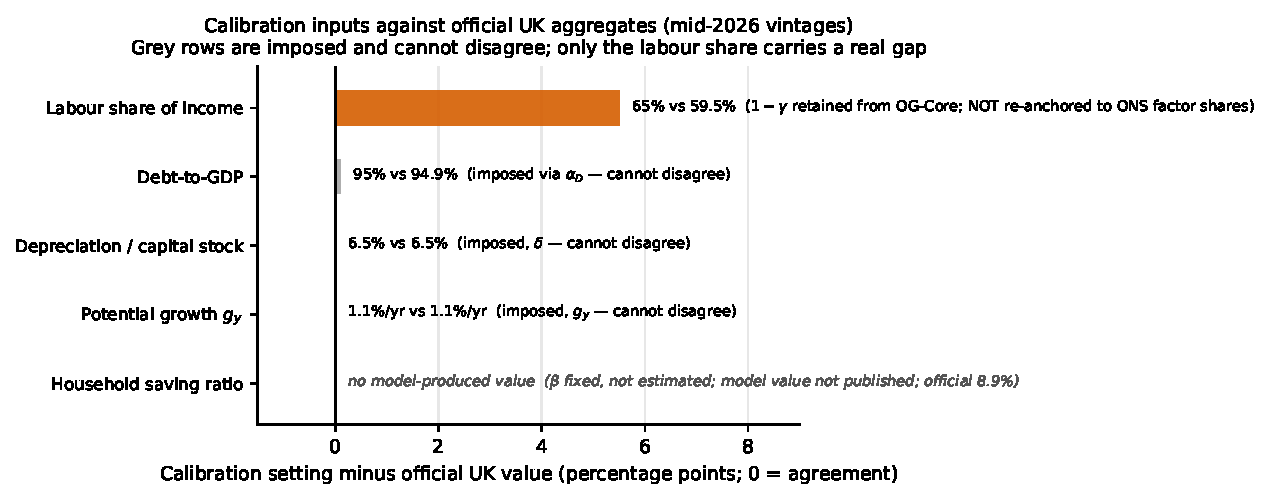
\includegraphics[width=0.92\textwidth]{figures/fig_targets.pdf}
\caption{Calibration targets against current official UK aggregates, each expressed as a percentage of the official value (dashed line = exact match). Annotations report the underlying values and the model treatment: an exact match on an \emph{imposed} or \emph{targeted} quantity is anchoring, not validation --- the over-identifying checks are the emergent ones (the capital--output ratio and the steady-state interest rate), for which no published reconciliation yet exists (Section~\ref{sec:limitations}).}
\label{fig:targets}
\end{figure}

The distinction in the treatment column matters for interpretation. Imposed quantities (depreciation, growth, the debt target) cannot disagree with the data; the genuinely over-identifying checks are the ones the steady state must \emph{deliver} --- the capital--output ratio and the interest rate consistent with the calibrated $(\gamma,\delta,\beta)$ triple. In the deployed fast configuration these emerge in an economically sensible range (a baseline steady-state real interest rate in low single digits, reported by \texttt{og-baseline} alongside the model-unit aggregates), but no systematic published reconciliation of achieved-versus-target moments exists for OG-UK 0.3.0, and this paper does not manufacture one: producing that reconciliation table from logged solves is the single most valuable next step for this member (Section~\ref{sec:limitations}). Two dating caveats on Table~\ref{tab:targets}: the official column reports the figures current at writing (mid-2026), while the deployed calibration was frozen against slightly earlier vintages; and the saving ratio is volatile quarter to quarter, so $\beta$ is matched to a smoothed level, not the latest print.

\subsection{Parameter choices against the OG-Core/OG-USA published defaults}
\label{subsec:paramcompare}

The second comparison is genealogical: OG-UK descends from OG-Core and its US calibration \citep{DeBackerEvans2024,DeBackerEvansOGUSA,DeBackerEvansPhillips2019}, so every departure of the deployed UK configuration from the published defaults is a deliberate, explicable choice. Table~\ref{tab:paramcompare} lays the two side by side.

\begin{table}[t]
\centering
\caption{Deployed OG-UK parameters against OG-Core/OG-USA published defaults}
\label{tab:paramcompare}
\resizebox{\textwidth}{!}{%
\begin{tabular}{llll}
\toprule
Parameter & OG-Core/OG-USA default & OG-UK deployed & Reason for deviation \\
\midrule
Frisch elasticity $\theta$ & 0.4 & 0.35--0.4 & UK/US macro-Frisch evidence \citep{BlundellMaCurdyMeghir2007,Peterman2016} \\
CRRA $\sigma$ & 1.5 & 1.5 & retained: standard value, no UK-specific estimate imposed \\
Discount factor $\beta$ (annual) & 0.96 & matched & re-targeted to the ONS household saving ratio, not fixed \\
Depreciation $\delta$ (annual) & 0.05 & 0.065 & ONS consumption of fixed capital / net stock ratio \\
Capital share $\gamma$ & 0.35 & $\approx 0.40$ & ONS national-accounts factor shares \\
Productivity growth $g_y$ (annual) & 0.03 & 0.011 & OBR potential-output growth: UK trend growth is far below the US default \\
Corporate tax rate $\tau^b$ & 0.21 (US statutory) & 0.27 effective & UK corporation-tax schedule \\
Consumption tax $\tau^c$ & 0 & VAT-anchored & the UK has a VAT; the US default abstracts from it \\
Ability types, shares $J$, $\lambda_j$ & 7; (.25,\,.25,\,.20,\,.10,\,.10,\,.09,\,.01) & unchanged & inherited; UK re-estimation is an open task (Section~\ref{sec:limitations}) \\
Ability profiles $e_{j,s}$ & US tax-microdata estimates & unchanged & inherited; the flagged limitation of Figure~\ref{fig:ability} \\
Tax-function form & DEP, age-specific \citep{DeBackerEvansPhillips2019} & Gouveia--Strauss, pooled & robustness over richness in the deployed fast configuration (Section~\ref{subsec:gs}) \\
Tax-function data & IRS/tax-calculator microdata & PolicyEngine UK on enhanced FRS & country substitution: the point of the OG-UK member \\
\bottomrule
\end{tabular}}
\end{table}

The deviations follow a single logic: quantities that describe the \emph{economy} (factor shares, depreciation, trend growth, tax rates, the microdata substrate) are re-anchored to UK sources, while quantities that describe \emph{preferences} ($\sigma$, the ability apparatus) are retained from the published US calibration unless UK evidence forces a change --- with the retained US ability profiles the flagged weak point. The largest single numerical departure is trend growth: the US default $g_y = 0.03$ would be indefensible for the UK, where the OBR puts potential growth near 1.1\% \citep{OBR2025EFO}, and since $g_y$ scales the entire balanced-growth path this one substitution changes long-run levels more than any preference parameter.

On the tax-function side, the published reference point is the DEP fit that \citet{DeBackerEvansPhillips2019} and the OG-USA documentation report for baseline US current law at age 42 in 2017: asymptotic maximum rates $max_x = 0.80$ ($max_x = 0.71$ for MTRx), fitted minimum rates of $-0.14$ to $-0.17$ (net transfer recipients), and a Cobb--Douglas income weight $\phi = 0.84$--$0.96$, estimated on 3{,}105 filer observations per rate. Figure~\ref{fig:depcompare} draws the schedules those published parameters imply and lays the paper's illustrative UK Gouveia--Strauss curve (the deployed functional form) alongside. The comparison is between \emph{published US fits} and an \emph{illustrative UK-shaped curve} --- no fitted UK parameter vector is published for OG-UK 0.3.0, and this paper does not manufacture one --- but it makes the structural point: both pipelines produce the same qualitative object, a smooth bounded schedule rising from near (or below) zero through the progressive range towards an asymptotic maximum, with the UK curve's faster early rise reflecting the personal-allowance taper and NICs arriving lower in the income distribution than the corresponding US thresholds.

\begin{figure}[t]
\centering
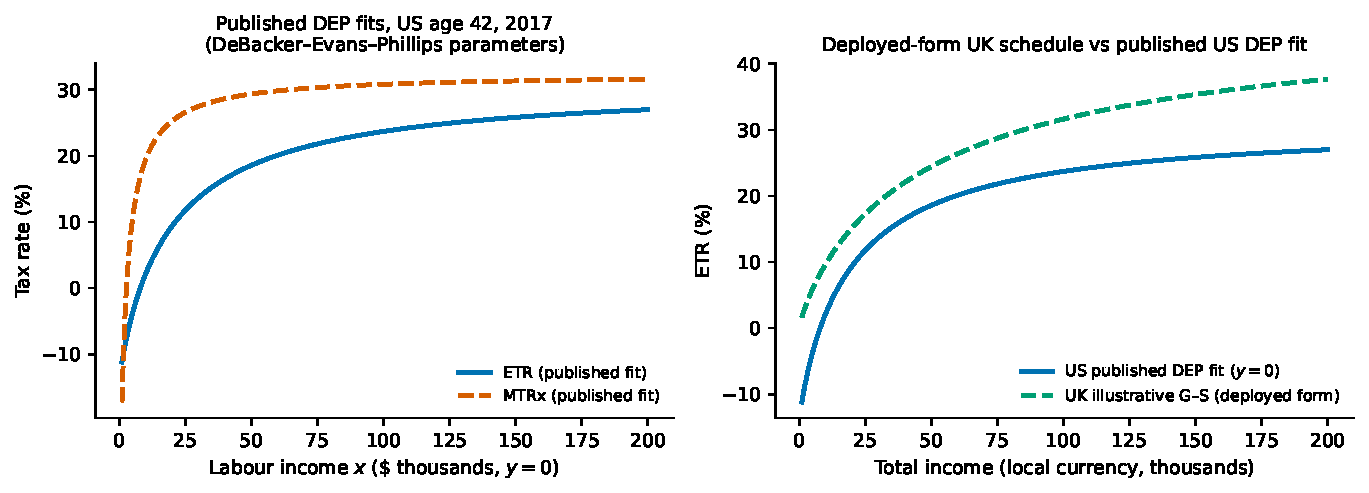
\includegraphics[width=\textwidth]{figures/fig_dep_compare.pdf}
\caption{Left: effective and marginal labour-income tax-rate schedules implied by the DEP parameter vectors published for baseline US current law, age 42, 2017 \citep{DeBackerEvansPhillips2019,DeBackerEvansOGUSA}, evaluated at zero capital income. Right: the published US ETR curve against this paper's illustrative UK Gouveia--Strauss ETR (the deployed functional form; not a fitted UK vector, which OG-UK 0.3.0 does not publish). Axes are in local-currency thousands; the comparison is qualitative by design.}
\label{fig:depcompare}
\end{figure}

\subsection{The OBR's UK OLG model as an external reference point}
\label{subsec:obrolg}

The closest published external reference is the OBR/HM Treasury UK OLG model of \citet{OBR2025OLG}: an independent codebase answering overlapping questions on the same economy. Table~\ref{tab:obrcompare} compares the two models' structure and calibration using the parameter values published in that working paper's calibration tables.

\begin{table}[t]
\centering
\caption{This paper's model (OG-UK as deployed) against the OBR's UK OLG \citep{OBR2025OLG}}
\label{tab:obrcompare}
\resizebox{\textwidth}{!}{%
\begin{tabular}{lll}
\toprule
 & OBR UK OLG (WP 22, April 2025) & OG-UK (this paper) \\
\midrule
Cohorts & ages 20--100 ($J=81$), annual & ages 20--99 ($S=80$), annual \\
Within-cohort heterogeneity & idiosyncratic persistent + transitory earnings shocks & 7 deterministic lifetime-ability types \\
Preferences & Cobb--Douglas CRRA, $\sigma_2 = 2$ & CRRA in consumption, elliptical labour disutility, $\sigma = 1.5$ \\
Discount factor & 0.99 (calibrated to WAS asset profile) & matched to ONS saving ratio \\
Frisch elasticity & $\approx$ 0.5 (0.3--0.5 to age 50, rising with age) & 0.35--0.4 (constant target) \\
Capital share & 0.33 & $\approx$ 0.40 \\
Depreciation & 5\% & 6.5\% \\
Productivity growth & 1.2\% (March 2024 EFO) & 1.1\% (OBR potential growth) \\
Debt-to-GDP target & 100\% & ONS-anchored ($\approx$ 95\%) \\
Tax detail & statutory rates and thresholds (March 2024) coded directly & smooth tax functions estimated from PolicyEngine microdata \\
Openness & closed baseline; open variant with $r^{*} = 5\%$ & closed baseline; open-economy features gilt-anchored \\
Bequests & warm glow, target \pounds 107,000, received at 55--75 & warm-glow intensity $\chi^b_j$, accidental bequests redistributed \\
\bottomrule
\end{tabular}}
\end{table}

The calibrations agree closely where both anchor to the same official sources (productivity growth 1.2\% vs 1.1\%; debt targets within a few points of current PSND) and differ where modelling philosophy differs: the OBR codes the statutory tax schedule directly and generates within-cohort inequality from earnings shocks, where OG-UK summarises the \emph{simulated} tax system --- benefit withdrawal included --- as smooth estimated functions and carries inequality through deterministic ability types. Neither is dominant: the OBR's shock-based heterogeneity produces precautionary saving that the deterministic-types model cannot, while the microdata-estimated tax functions capture effective-rate detail (the UC taper, the \pounds 100,000 allowance withdrawal) that coded statutory schedules of the marginal-rate-and-threshold kind omit.

On results, the overlap currently available is qualitative. WP 22's headline policy experiment is exactly the reform class this paper uses as its running example --- a 1 percentage point change in the basic rate of income tax --- for which the OBR model delivers a long-run GDP fall of 0.1\%, a 0.2\% fall in total hours (concentrated at ages above 50), and an income-tax yield of roughly \pounds 8bn ($\approx$ 0.3\% of GDP), with a near-symmetric response to a cut. Those are steady-state, closed-economy, full-anticipation numbers --- the same experiment type as this member's CLI scoring --- and they provide the natural external benchmark: an OG-UK basic-rate score whose signs match (output and hours down, revenue up by somewhat less than the static yield) and whose magnitudes fall in the same sub-half-percent range would be corroborating; a materially larger response would point first at the Frisch calibration and the estimated MTR schedules. WP 22 publishes no steady-state capital--output ratio or long-run elasticity table beyond these scenario results, so a full quantitative reconciliation is not yet possible from published numbers alone; producing the OG-UK side of this comparison from logged solves is part of the validation agenda of Section~\ref{sec:limitations}.
